\documentclass{standalonex}
\usepackage{tikz}

\begin{document}
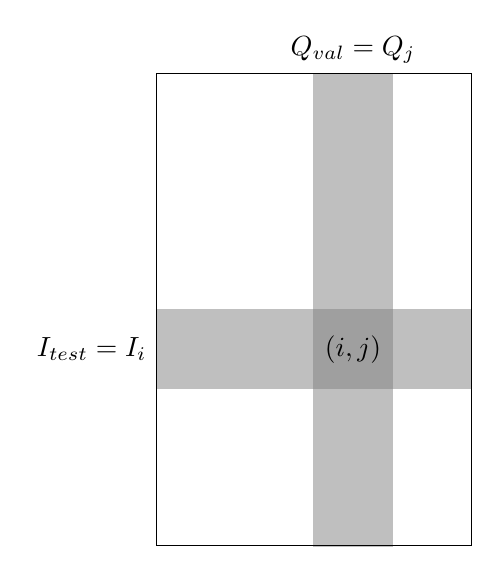
\begin{tikzpicture}
\filldraw[help lines,opacity=0.5] (0,2) rectangle ++(4,1);
\filldraw[help lines,opacity=0.5] (2,0) rectangle ++(1,6);
\node at (2.5,2.5) {$(i, j)$};
\node[above] at (2.5,6) {$Q_{val} = Q_j$};
\node[left] at (0,2.5) {$I_{test} = I_i$};
\draw (0,0) rectangle (4,6);
\end{tikzpicture}
\end{document}
